\documentclass[sigconf]{acmart}

\usepackage{booktabs} % For formal tables

\newcounter{myctr}
\newenvironment{compactEnumerate}{\begin{list}{\arabic{myctr}.}
{\usecounter{myctr}
%\setlength{\topsep}{1mm}\setlength{\itemsep}{0.5mm}
\setlength{\topsep}{0.3mm}\setlength{\itemsep}{0mm}
\setlength{\parsep}{0.3mm}
\setlength{\itemindent}{0mm}\setlength{\partopsep}{0mm}
\setlength{\labelwidth}{15mm}
\setlength{\leftmargin}{4mm}}}{\end{list}}

% Copyright
%\setcopyright{none}
\setcopyright{acmcopyright}
%\setcopyright{acmlicensed}
%\setcopyright{rightsretained}
%\setcopyright{usgov}
%\setcopyright{usgovmixed}
%\setcopyright{cagov}
%\setcopyright{cagovmixed}


\copyrightyear{2019} 
\acmYear{2019} 
%\setcopyright{acmlicensed}
\acmConference[DAC '19]{The 56th ACM/ESDA/IEEE Design Automation Conference}{June 2--6, 2019}{Las Vegas, USA}
%\acmBooktitle{The 34th ACM/SIGAPP Symposium on Applied Computing (SAC '19), April 8--12, 2019, Limassol, Cyprus}
%\acmPrice{15.00}
%\acmDOI{10.1145/3297280.3297337}
%\acmISBN{978-1-4503-5933-7/19/04}



%\acmArticle{4}
%\acmPrice{15.00}

% These commands are optional
%\acmBooktitle{Transactions of the ACM Woodstock conference}
%\editor{Jennifer B. Sartor}
%\editor{Theo D'Hondt}
%\editor{Wolfgang De Meuter}

%%%%%%%%%%%%%%%%%%%%%%%%%%%%%%%%%%%%%%%%%%%%%%%%%%%%

\usepackage{amsmath}
\usepackage{amssymb}
\usepackage{subcaption}
\usepackage{multicol}
\usepackage[inline]{enumitem}

\newcommand{\todo}[1]{{\emph{TODO: #1}}}
\newcommand{\martin}[1]{{\color{blue} Martin: #1}}
\newcommand{\marten}[1]{{\color{cyan} Marten: #1}}
\newcommand{\isa}[1]{{\color{darkgreen} Isabelle: #1}}


%% uncomment following for final submission
%\renewcommand{\todo}[1]{}
%\renewcommand{\martin}[1]{}
%%\renewcommand{\benjamin}[1]{}
%\renewcommand{\isa}[1]{}

\begin{document}

\title{Actors, Time Stamps, and Determinism \\ for Time-Critical Systems}


\author{Marten Lohstroh}
\orcid{0000-0001-8833-4117}
\email{marten@eecs.berkeley.edu}
% \affiliation{%
% 	\institution{University of California, Berkeley}
% 	%\streetaddress{}
% 	%\postcode{}
% 	%\city{} 
% 	\country{USA} 
% }

\affiliation{%
	\institution{UC Berkeley, USA}
	%\streetaddress{}
	%\postcode{}
	%\city{} 
	% \country{USA} 
}

\author{Martin Schoeberl}
\orcid{1234-5678-9012}
\email{masca@dtu.dk}
\affiliation{%
	\institution{TU Denmark, Denmark}
	%\streetaddress{}
	%\postcode{2800}
	%\city{Lyngby} 
	% \country{Denmark} 
}

\author{Andr\'es Goens}
\orcid{}
\email{andres.goens@tu-dresden.de}
\affiliation{%
	\institution{TU Dresden, Germany}
	%\streetaddress{}
	%\postcode{}
	%\city{} 
	% \country{USA} 
}

\author{Armin Wasicek}
\orcid{}
\email{armin.wasicek@avast.com}
\affiliation{%
	\institution{Avast, USA}
	%\streetaddress{}
	%\postcode{}
	%\city{} 
	%\country{USA} 
}

\author{Christopher Gill}
\orcid{}
\email{cdgill@wustl.edu}

\affiliation{%
	\institution{Washington Univ., St. Louis, USA}
	%\streetaddress{}
	%\postcode{}
	%\city{} 
	%\country{USA} 
}

\author{Marjan Sirjani}
\orcid{}
\email{marjan.sirjani@mdh.se}

\affiliation{%
	\institution{M\"alardalen Univ., Sweden}
	%\streetaddress{}
	%\postcode{}
	%\city{} 
	%\country{Sweden} 
}

\author{Edward A. Lee}
\orcid{0000-0002-5663-0584}
\email{eal@eecs.berkeley.edu}

\affiliation{%
	\institution{UC Berkeley, USA}
	%\streetaddress{}
	%\postcode{}
	%\city{} 
	%\country{USA} 
}


\renewcommand{\shortauthors}{E. A. Lee et al.}

\begin{abstract}
Abstract
\end{abstract}

%
% The code below should be generated by the tool at
% http://dl.acm.org/ccs.cfm
% Please copy and paste the code instead of the example below. 
%
\begin{CCSXML}
	<ccs2012>
	<concept>
	<concept_id>10010520.10010553.10010562</concept_id>
	<concept_desc>Computer systems organization~Embedded systems</concept_desc>
	<concept_significance>500</concept_significance>
	</concept>
	</ccs2012>  
\end{CCSXML}

\ccsdesc[500]{Computer systems organization~Embedded systems}

\keywords{ACM proceedings, \LaTeX, text tagging}%

\ccsdesc[500]{Computer systems organization~Embedded systems}


\keywords{actor, real-time systems, worst-case execution time}

\maketitle 


\section{Introduction}\label{sec:intro}
Since their introduction by Hewitt~\cite{Hewitt:77:Actors} in the 70s, the use of actors has proliferated 
in programming languages~\cite{Armstrong:96:Erlang,haller2009scala,desai2013p}, coordination languages~\cite{Arbab:04:Reo,ARC}, distributed systems~\cite{Hunt2018, DBLP:journals/corr/abs-1712-05889}, and simulation engines~\cite{Ptolemy:14:Book,DBLP:journals/fuin/SirjaniMSB04}. 
Actors have much in common with objects---a paradigm focused on reducing code replication 
by means of inheritance and increasing modularity via data hiding---but unlike %the Object Oriented Programming (OOP) paradigm
objects, actors also provide a model for \emph{concurrency}. 
Indeed, in the original formulation of the actor model, each actor is presumed to operate concurrently alongside
other actors that it may exchange messages with, asynchronously. The lack of any guarantees
with respect to the ordering of messages, and the absence of a notion of time, makes this a
very general model, but not a very useful model for the specification of systems in which
timely execution and determinism are important. While precision timing plays an important role
in control systems that continually interact with concurrent physical processes (i.e., cyber-physical
systems), determinism makes \emph{any} software easier to test and verify.

Extra machinery can be introduced for the formal specification and analysis of systems composed of Hewitt actors.
For instance, Real-time Maude~\cite{olveczky:2008:real}, a timed rewriting logic framework and (temporal) model checking tool, has been applied to actors in~\cite{Ding2003}. Similarly, the modeling language Rebeca performs analysis that uses a model checker to ensure that nondeterminism allowed in the model does not lead to behaviors that violate requirements of the simulated system~\cite{DBLP:conf/birthday/SirjaniJ11} \marten{this doesn't appear to be the correct reference}. Alternatively, constraints can be placed on actors' allowable behaviors so that they adhere to a well-defined model of computation (MoC), satisfying desirable properties such as deadlock freedom, schedulability, bounded memory usage, and deterministic execution by construction. It is the latter approach we follow. In this paper, we propose a programming model that ensures that messages between actors are handled in deterministic order unless nondeterminism is introduced explicitly. We introduce \emph{Lingua Franca} (LF), an interface definition language for the description of actors and their composition. By default, all Lingua Franca programs will be deterministic. We use a semantic notion of time and time stamps to achieve this.

\section{Actors in Lingua Franca}\label{sec:actor}
A key difference between Hewitt's notion of actors and actors in LF, is that rather than having actors address other actors directly, LF actors send messages via ports, completely agnostic of the presence or absence of downstream receivers. The connections between actors are embedded in a level of hierarchy---a composite---that is tasked with relaying messages between contained actors. While this approach increases modularity, more importantly, \marten{it exposes dependencies between actors that can be exploited...
discuss DE, SR, performance.}

\marten{Inspired by \cite{LeeMatsikoudis:09:Dataflow}, reaction rules, etc...

Note that because a dependency graph can be derived from the component interfaces and topology, no static analysis has to be performed on the code that implements the reactions in order to construct a schedule. This is why LF can be polyglot...}

Central to the programming model behind LF is the relationship between the time stamps associated with the receipt of messages, which denote \emph{logical} time, and the passing of \emph{physical} time, approximated by the system time of the execution platform. While logical time can be sped up or slowed down arbitrarily a simulation, the fact that actors can interact with the physical world through sensors and actuators requires that logical time and physical time ``keep up'' with one another in order to have a temporal semantics that obeys the principle of causality (i.e., effects cannot precede causes) for all observers. 

% Time is \emph{logical} time. This logical time be used for simulation and then
% we call it model time. We can also use the network of actors for the implementation
% of the system. 

% In that case wall clock time is used to timestamp input values
% at sensors. Logical time can never advance further than wall clock time.
% We have a notion of delay in two places: (1) as a delay actor to break up
% feedback loops (2) at actuators to specify that an actuation shall happen before
% (or exactly at) the logical time of the input plus the delay.

% Actors communicate via ports. All data exchanged has a timestamp.
% An actor does not advance time, the reaction is considered instantaneous.

% Reactions of one actor are atomic and are allowed to change state.
% Reactions are triggered by available inputs with timestamps at logical
% time (or older). When several reactions of an actor are enabled at the
% same time, the definition order in LF defines the execution order.

% A reaction of an actor can also be released by a trigger. A trigger
% can be periodic triggers or a single shot timer.


\begin{enumerate}
\item Messages exchanged between actors are timestamped;
\item The arrival of a message denotes a discrete event;
\item Actors carry state and a list of reactions, each of which:
\begin{enumerate}
\item is triggered by the presence of an event;
\item sees events in time stamp order;
\item can read/modify the actor's state;
\item can set the values of output ports it has access to;
\item can schedule \emph{future} events on input ports it has access to;
\item can read the values of input ports it has access to;
\begin{enumerate}
\item the timestamp associated with an observed event always denotes the current logical time; and
\item if no message arrived at a given port at the current logical time, its observed value is \emph{absent}. 
\end{enumerate}
\end{enumerate}
\item No logical time elapses during a reaction;
\item Any two reactions of the same actor execute atomically with respect to one another; and
\item If two reactions of the same actor are triggered simultaneously, they execute in a predefined order;
\end{enumerate}

% 

%This paper is organized as follows. Section~\ref{sec:related} surveys related work.
%Section~\ref{sec:hardware} describes the proposed time-predictable branch predictor
%and its different variations. Section~\ref{sec:wcet} presents the associated scope-based
%static WCET analysis technique. Section~\ref{sec:eval} analyzes the worst-case behavior
%of the proposed branch predictor. Finally, Section~\ref{sec:conclusion} concludes
%and gives directions for future work.

\section{A Motivating Example}

\subsection{Deadlines}
\begin{figure}[ht]
 \centering
 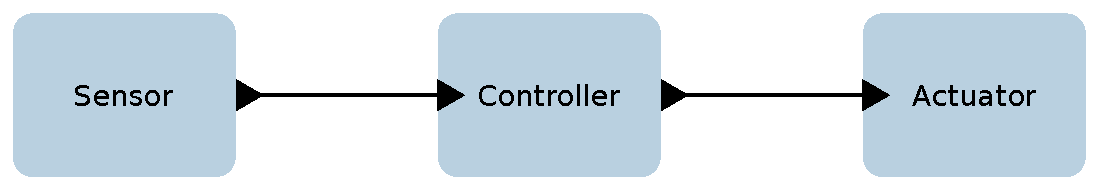
\includegraphics[width=\linewidth]{img/example-1}
 \caption{First example}
 \label{fig:example-1}
\end{figure}
% DAC Properties A1-9.
% Simple examples. Which should those be?
% First one to start with: sensor computation actuator
% Introduce notion of a deadline
% Why on the local platform, model should not get ahead.
% Example 1: Synchronization to real time and deadlines
% Example 2: Why delay has to wait
% Example 3: shut off the lights some time after the switch has been flipped.
% Reason to have the deadline definition as stated: detectability. Suppose the start deadline cannot be met; the
% reaction should not be carried out (and then the violation be reported on).

\subsection{Causality}
We don't want to run ahead of realtime, because actors can produce spontaneous events that need to be stamped with 
pysical time, and we don't want these timestamps to be ``in the past.''

\begin{figure}[ht]
 \centering
 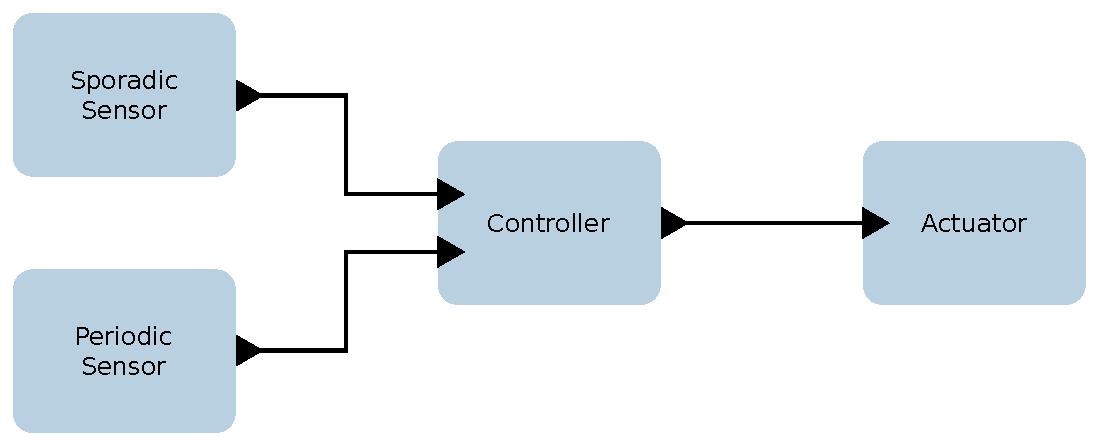
\includegraphics[width=\linewidth]{img/example-2}
 \caption{Second example}
 \label{fig:example-2}
\end{figure}


\subsection{}
Shut off the lights some time after the switch has been flipped. Reason to have the deadline definition as stated: detectability. Suppose the start deadline cannot be met; the reaction should not be carried out (and the violation be reported on subsequently).

\begin{figure}[ht]
 \centering
 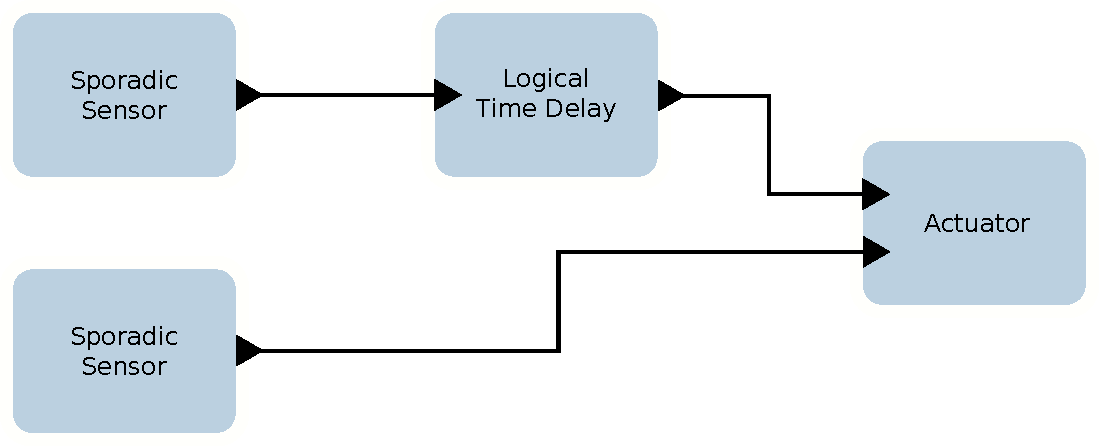
\includegraphics[width=\linewidth]{img/example-3}
 \caption{Third example}
 \label{fig:example-3}
\end{figure}

\section{Related Work}
\label{sec:related}
Towards a real-time coordination model for mobile computing \cite{hackmann2005towards}
Method and tools for mixed-criticality real-time applications within PharOS \cite{lemerre2011method}
Accessors \cite{brooks2018component}
S-Net~\cite{grelck2008gentle}
%\section{Actors}
%


% Constraints can be placed on actors' allowable behaviors so that actors adhere to a well-defined model of computation, satisfying desirable properties such as deadlock freedom, schedulability, bounded memory usage, and deterministic execution by construction. This has been the guiding principle in the Ptolemy project\footnote{\url{https://ptolemy.berkeley.edu/}}, which studies modeling, simulation, and design of concurrent, real-time, embedded systems.

% Several frameworks have been built based, loosely or strictly, on the
% original Hewitt actor model
% \cite{Hewitt:77:Actors,Agha:97:ActorComputation}, including Akka
% \cite{AkkaAction2016},
% Ray \cite{DBLP:journals/corr/abs-1712-05889}, and Rebeca
% \cite{DBLP:journals/fuin/SirjaniMSB04}. One property of the original
% Hewitt actor model is that messages received by an actor from distinct
% sources are handled in nondeterministic order. \marten{even messages from the same source can arrive out-of-order}


% \martin{We need to check this: Outputs generated by a time triggered
% reaction are timestamped. When the system is simulated, the timestamp
% is equal to the model time. When the system is used for execution, the logical
% time for the release of the reaction is synchronized to wall clock time and therefore
% the output message are synchronized to wall clock time.}

\martin{Question: what happens when a reaction depends on two inputs, but
those two inputs have a different logical time?
I assume that the reaction is fired/released when all two inputs have values
(which means logical time is at the younger message)
and a produced output gets the younger timestamp.}
\marten{It cannot happen. As discussed earlier: we should probably discuss persistent ports as a feature to facilitate writing actors that relate messages with different timestamps.}

% \martin{We have (and maybe support) two options: (1) input is only valid when
% the timestamp equals logical time, absent at other times or (2) keeping the value
% of an input for future logical time and having a default value for system initialization time.
% (in the JS accessors this is the way it is specified, the default value gives the
% ``keep'' or persistent semantic).}

\subsection{Scribbles on Logical Time}
Time is \emph{logical} time. This logical time be used for simulation and then
we call it model time. We can also use the network of actors for the implementation
of the system. In that case wall clock time is used to timestamp input values
at sensors. Logical time can never advance further than wall clock time. \marten{Not entirely true: an optimized scheduler can do this under very specific circumstances that we'll elaborate on in the example.}
We have a notion of delay in two places: (1) as a delay actor to break up
feedback loops (2) at actuators to specify that an actuation shall happen before
(or exactly at) the logical time of the input plus the delay.

The scheduler invokes reactions of actors dependent in inputs with timestamps
that are equal (or earlier--can this happen?) at logical time $t_1$.
Logical time cannot advance further than wall clock time $t_w$. If next logical
time $t_2 > t_w$ the scheduler waits till $t_w \ge t_2$.

\subsection{Sporadic Events and Call Backs}

Sporadic events and call backs can trigger a reaction. This reaction is allowed
to observe and also change the state of the actor. Therefore, they are not allowed
to preempt a reaction (reactions are atomic to each other). To enforce this atomicity
a sporadic reaction is executed only between two logical timestamps $t_1$ and $t_2$.
This can be enforced on a C based host by turning off interrupts when executing
a reaction. Interrupts are enabled when all\footnote{\todo{All is a little bit restrictive,
just for state atomicity we would not need to wait for all reaction, just for a single.
But there is another issue that this shall happen only between two timestamps.
I don't recall the details.}}
reactions for timestamp $t_1$ have been executed and disabled again when logical
time is advanced to $t_2$ where all reactions for $t_2$ are executed.


\todo{Describe that the single threaded execution of JavaScript enforces
the restriction of the call back not interrupting the reaction.}

\subsection{More Scribbles}

Delays deserve also the purpose to align events with wall clock time and to
allow execution of reactions in their worst-case execution time (WCET).
The summ of all reaction's WCET from one synchronization point (either
sample of sensors or output of a delay actor) to another synchronization
point (or output of an actuator) has to be less than the delay.

\subsection{Dynamic Actors}

For dynamic systems, e.g., an IoT that keeps running, but in different contexts
(e.g., places), we support dynamic reconfiguration of the network of actors.
This may be well supported when targeting a dynamic language such as JavaScript,
but harder to implement in C.

To support reconfiguration we need a more complete language then the configuration
language LF. Therefore, our first iteration of dynamic reconfiguration is done in the
host language JavaScript. In that case, the host language needs access to actors and
ports. However, we can use scopes to having access to those parts of the framework
only in well defined places.

\subsection{Call of an External Service}

An actor can call an external service that will deliver the result in the future
and use a call back to deliver the result (\martin{Marten likes to use a Future}).
This call back is handled as described above between two model timestamps
and the return value is timestamped with wall clock time.

An actor my implement a timeout mechanism by scheduling a trigger in the future.
{\bf This timeout TO need to be set relative to wall clock time, not logical
time, as logical time will be behind wall clock time.}



\section{Conclusion}
\label{sec:conclusion}


\subsection*{Acknowledgment}

%The work presented in this paper was partially funded by the
%Danish Council for Independent Research \textbar{} Technology and Production Sciences
%under the project PREDICT\footnote{\url{http://predict.compute.dtu.dk/}}
%contract no.~4184-00127A.

% Please do not add any references to msbib.bib.
% They get lost when I 'generate' it again.
\bibliographystyle{ACM-Reference-Format}
\bibliography{Refs} 

\end{document}
